\let\negmedspace\undefined
\let\negthickspace\undefined
\documentclass[journal]{IEEEtran}
\usepackage[a5paper, margin=10mm, onecolumn]{geometry}
\usepackage{lmodern} 
\usepackage{tfrupee} 
\setlength{\headheight}{1cm}
\setlength{\headsep}{0mm}   

\usepackage{gvv-book}
\usepackage{gvv}
\usepackage{cite}
\usepackage{amsmath,amssymb,amsfonts,amsthm}
\newcommand{\augvec}[3]{%
  \left(\begin{array}{*{#1}{c}|*{#2}{c}}
  #3
  \end{array}\right)}

\usepackage{algorithmic}
\usepackage{graphicx}
\usepackage{textcomp}
\usepackage{xcolor}
\usepackage{txfonts}
\usepackage{listings}
\usepackage{enumitem}
\usepackage{mathtools}
\usepackage{gensymb}
\usepackage{comment}
\usepackage[breaklinks=true]{hyperref}
\usepackage{tkz-euclide} 
\usepackage{listings}                             
\def\inputGnumericTable{}                                 
\usepackage[latin1]{inputenc}                                
\usepackage{color}                                            
\usepackage{array}                                            
\usepackage{longtable}                                       
\usepackage{calc}                                             
\usepackage{multirow}                                         
\usepackage{hhline}                                           
\usepackage{ifthen}                                           
\usepackage{lscape}
\usepackage{xparse}

\bibliographystyle{IEEEtran}

\title{5.2.61}
\author{EE25BTECH11059 - Vaishnavi Ramkrishna Anantheertha}

\begin{document}
\maketitle

\renewcommand{\thefigure}{\theenumi}
\renewcommand{\thetable}{\theenumi}

\numberwithin{equation}{enumi}
\numberwithin{figure}{enumi} 

\textbf{Question}:
Solve the system:\\
  x - y + 2z = 1 \\
   2z - 3z = 1 \\
  3x - 2y + 4z = 2


\textbf{Solution }
\begin{table}[H]    
  \centering
  \begin{tabular}{|c|c|}
\hline
\textbf{Name} & \textbf{Value} \\ \hline
$\vec{A}$ & $\myvec{2 & 1 \\0 & 3}$ \\ \hline
\end{tabular}

  \caption{Variables Used}
  \label{tab:4.7.56}
\end{table}
\begin{align}
    \myvec{1 & -1 & 2}\Vec{X}=1\\
     \myvec{0 & 2 & -3}\Vec{X}=1\\
      \myvec{3 & -2 & 4}\Vec{X}=2
\end{align}
This system of equations can be solved using an augmented matrix 
\begin{align}
\augvec{3}{1}{
1 & -1 & 2 & 1 \\
0 & 2 & -3 & 1 \\
3 & -2 & 4 & 2}
&\xrightarrow{R_3 \to R_3 - 3R_1}
\augvec{3}{1}{
1 & -1 & 2 & 1 \\
0 & 2 & -3 & 1 \\
0 & 1 & -2 & -1} \\[6pt]
&\xrightarrow{R_3 \to R_3 - \tfrac{1}{2} R_2}
\augvec{3}{1}{
1 & -1 & 2 & 1 \\
0 & 2 & -3 & 1 \\
0 & 0 & -\tfrac{1}{2} & -\tfrac{3}{2}} \\[6pt]
&\xrightarrow{R_2 \to \tfrac{1}{2} R_2}
\augvec{3}{1}{
1 & -1 & 2 & 1 \\
0 & 1 & -\tfrac{3}{2} & \tfrac{1}{2} \\
0 & 0 & -\tfrac{1}{2} & -\tfrac{3}{2}} \\[6pt]
&\xrightarrow{R_3 \to -2 R_3}
\augvec{3}{1}{
1 & -1 & 2 & 1 \\
0 & 1 & -\tfrac{3}{2} & \tfrac{1}{2} \\
0 & 0 & 1 & 3} \\[6pt]
&\xrightarrow{R_2 \to R_2 + \tfrac{3}{2} R_3}
\augvec{3}{1}{
1 & -1 & 2 & 1 \\
0 & 1 & 0 & 5 \\
0 & 0 & 1 & 3} \\[6pt]
&\xrightarrow{R_1 \to R_1 - 2R_3}
\augvec{3}{1}{
1 & -1 & 0 & -5 \\
0 & 1 & 0 & 5 \\
0 & 0 & 1 & 3} \\[6pt]
&\xrightarrow{R_1 \to R_1 + R_2}
\augvec{3}{1}{
1 & 0 & 0 & 0 \\
0 & 1 & 0 & 5 \\
0 & 0 & 1 & 3} \\[6pt]
      \Vec{X}=\myvec{0
                    \\
                     5
                    \\
                     3}\\
&x = 0, \quad y = 5, \quad z = 3
\end{align}





Refer to Figure

\begin{figure}[H]
\begin{center}
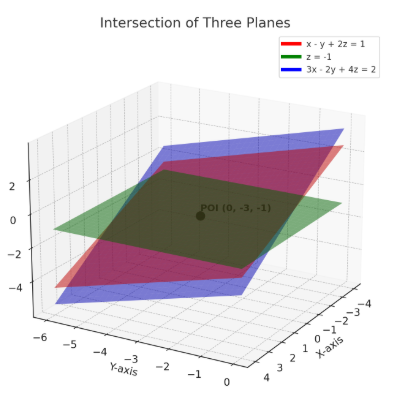
\includegraphics[width=0.6\columnwidth]{figs/graph9.png}
\end{center}
\caption{}
\label{fig:Fig}
\end{figure}
\end{document}